% % % % % % % % % % % % % % % % % % % % % % % % % % % % % % % % % % % % %
% Chapter: Test mechanics
% % % % % % % % % % % % % % % % % % % % % % % % % % % % % % % % % % % % %
\chapter{Test mechanics}
\label{cpt:testmechanics}
\pinfo{Intro, describing contents of chapter}
In order to check whether these properties hold when using the generator, we
need to determine how the test framework should work. In this chapter we will
try to answer the following research question:
\begin{description}
  \item [RQ 2:] \rqTwo
\end{description}

We use property-based testing as testing technique. The aim of this project is
to test the implementation of the generator and trying to find yet unknown bugs
in it. Unfortunately we cannot test the properties right away on the generator,
but we aim to test the properties as automatic as possible. To check the
generator, we need to use the system that it generates. But in order to do this,
a valid \textit{Rebel} specification is required. In this chapter we describe
how the test framework is setup such that it can automatically check whether the
defined properties hold when using the generator.

% % % % % % % % % % % % % % % % % % % % % % % % % % % % % % % % % % % % %
% Section: The test framework
\section{The test framework}
\pinfo{Describing phases}
A \textit{Rebel} specification can be created with the property definitions.
Which can then be used to generate the test cases. The collection of resulting
test cases is the content of the test suite, which we can be run against the
generated system. We can divide the process into different phases. The goal of
the test framework is to combine most of the required phases such that each
defined property is being checked as automatic as possible. An overview of the
phases is shown in Figure X, to sum up: the phases
are defined as follows:
\def \tfPhaseOne{Create specification}
\def \tfPhaseTwo{Check \& Build}
\def \tfPhaseThree{Generate system}
\def \tfPhaseFour{Generate test suite}
\def \tfPhaseFive{Run test suite}
\begin{enumerate}
  \item \tfPhaseOne{}
  \item \tfPhaseTwo{}
  \item \tfPhaseThree{}
  \item \tfPhaseFour{}
  \item \tfPhaseFive{}
\end{enumerate}

We will describe each phase in detail in the next sections. Additionally we will
define some evaluation criteria which will be used to evaluate the test
framework. The \textit{Reflexitivity} property will be used to demonstrate each
phase. More specifically: the case of \textit{Reflexivity} when using equality,
called \textit{ReflexiveEquality} throughout this project. The definition of
\textit{ReflexiveEquality} is shown in
\autoref{tbl:ch3_small_property_definition}.
% Table
\FloatBarrier
\begin{table}[!ht]
\centering
\begin{tabular}{ccc}
\hline
% \multicolumn{3}{c}{\textbf{ReflexiveEquality}} \\ \hline
\textbf{Formula} & \textbf{Variable} & \textbf{Type} \\ \hline
x == x & x & Money \\ \hline
\end{tabular}
\caption{Property definition of \textit{ReflexiveEquality}}
\label{tbl:ch3_small_property_definition}
\end{table}
\FloatBarrier
% End table

% % % % % % % % % % % % %
% Subsection: From property definitions to Rebel specification
\subsection{\tfPhaseOne{}}
\label{sct:3_prop_to_rebel}
\pinfo{Generator requires spec}
The generator requires a consistent \textit{Rebel} specification in order to generate a system. This means that we have to translate the properties (which are defined in \autoref{cpt:properties}) to a \textit{Rebel} specification. A rebel specification consist of a lifecycle definition together with its event definitions.\\
\\
\pinfo{Property to event translation}
A test case should be able to pass values as parameters to test a specific property for a certain amount of times. We can use the events for this in the \textit{Rebel} definition. An event describes a transition from one state to another and accepts parameters. Additionally, it can have pre- and postconditions, where the postconditions can state what happens when the transaction is being executed. In \autoref{lst:ch3_rebel_event_of_property} the event definition for the \textit{ReflexiveEquality} property written in \textit{Rebel} is shown.
% Listing
\FloatBarrier
\begin{sourcecode}[!ht]
\begin{lstlisting}[language=Rebel]
event reflexiveEquality(x: Money) {
    postconditions {
       new this.result == ( x == x );
    }
}
\end{lstlisting}
\caption{The event definition for the \textit{ReflexiveEquality} property.}
\label{lst:ch3_rebel_event_of_property}
\end{sourcecode}
\FloatBarrier
% End listing
\pinfo{Further explanation, parameters, result field}
The event name and the parameters are used to generate a test case from this event definition. To check whether the property was fulfilled given a certain tuple of parameters, we store the result in a data field called \textit{result}. The test cases can retrieve the value of this field, to determine the result. In case the result value is \textit{false} during testing, a bug has been found. (The \textit{new} keyword is used to state how the field changes when a transition is taking place.)\\
\\
\pinfo{Also need to define the specification itself}
Besides the event definition, we need to write the actual \textit{Rebel} specification to be able to generate a system from it. The specification describes the fields, the events it uses and the life cycle of the state machine. Since we are only interested in testing the events, we can hold the specification itself to a minimum. The life cycle consists of 2 states, the initial and final state. The transition between these states is the event we defined, \textit{ReflexiveEquality}. In \autoref{lst:ch3_rebel_specification_oneprop} a specification used for one property is shown. In the case of multiple properties, we can add these to the events block. In the life cycle, we can comma separate the transitions.
% Listing
\FloatBarrier
\begin{sourcecode}[!ht]
\begin{lstlisting}[language=Rebel]
module gen.specs_money.MoneyExample

import gen.specs_money.MoneyExampleLibrary

specification MoneyExample {
	fields {
        id: Integer @key
		result: Boolean
	}

	events {
		reflexiveEquality[]
	}

	lifeCycle {
		initial init -> result:	reflexiveEquality
		final result
	}
}
\end{lstlisting}
\caption{The event definition for the \textit{ReflexiveEquality} property.}
\label{lst:ch3_rebel_specification_oneprop}
\end{sourcecode}
\FloatBarrier
% End listing

% % % % % % % % % % % % %
% Subsection: Phase 2: Check & build
\subsection{\tfPhaseTwo{}}
\pinfo{Build specification}
Now that we have a specification, that specification can be checked and builded. Which results in an AST of the specification that the test framework can use to generate the tests. This is done by using the existing toolchain that is available for Rebel. The test framework itself is written in \textit{Rascal}.\\
\\
\pinfo{Building to AST}
Building the specification means that the specification is being checked and returns an AST of the specification when the specification is consistent. This is required in order to generate a system from it by using the generator, additonally the AST is used by the test framework to generate the test suite.

% % % % % % % % % % % % %
% Subsection: Phase 3: Generate system
\subsection{\tfPhaseThree{}}
\pinfo{SUT is the generated system}
The generator will be used to generate a system from the specification that we have created. This system which will be used to check each property and is called the SUT throughout this thesis. Note that the generated system is assumed to be runnable. As otherwise the test suite, that will be generated by the test framework (in the next phase), cannot be run against the generated system.

% % % % % % % % % % % % %
% Subsection: Phase 4: Generate test suite
\subsection{\tfPhaseFour{}}
\label{sct:3_tf_phase_four}
\pinfo{Init and generate}
The test suite requires some configuration to work with the generated system. The test framework first initializes the test suite, then generates the test cases.\\
\\
\pinfo{Test suite initialization}
The generated system uses Akka as messaging layer, the required configuration files for running the test suite on the generated system are added by the test framework. Furthermore the test suite is build up such that it first starts the SUT and then runs all the tests against the SUT. Thus when running the test suite (next phase), the SUT will automatically be started such that this does not require additional steps. Furthermore the initialization part can be found back in the source of this project. We do not cover this in detail here since there are no custom settings in there, rather its more default configuration that is only required to make the messaging layer work for the test suite.\\
\\
\pinfo{Test case generation based on event}
The test framework can traverse the AST and generate a test case for each event. A test case is generated by using the templating feature of Rascal, where we fill in event specific data as shown in \autoref{lst:ch3_rascal_testcase_template}. The resulting test case of \textit{ReflexiveEquality} is shown in \autoref{lst:ch3_generated_test_example}.
% Listing
\FloatBarrier
\begin{sourcecode}[!ht]
\begin{lstlisting}[language=Rascal]
public str snippetTestCase(str eventName, list[str] params, int tries) {
	return "\"work with <eventName>\" in {
	          generateRandomParamList(<convertParamsToList(params)>, <tries>).foreach {
	            data: List[Any] =\> {
	              checkAction(<eventName>(
	       	        <for (i <- [0..size(params)]) {>
                      // Iterate over params. Use getMappedType for the casting again
                      data(<i>).asInstanceOf[<getMappedTypeForParam(params[i])>]
                      // Add a comma if needed
                      <if (i != size(params)-1) {>,<}>
                    <}>
	                )
	              )
	            }
	          }
	        }";
}
\end{lstlisting}
\caption{Test case snippet}
\label{lst:ch3_rascal_testcase_template}
\end{sourcecode}
\FloatBarrier
% End listing

% Listing
\FloatBarrier
\begin{sourcecode}[!ht]
\begin{lstlisting}[language=Scala]
    "work with ReflexiveEquality" in {
       generateRandomParamList(List("Money"), 100).foreach {
         data: List[Any] => {
           checkAction( ReflexiveEquality(data(0).asInstanceOf[Money]) )
         }
       }
     }
\end{lstlisting}
\caption{An example of a generated test}
\label{lst:ch3_generated_test_example}
\end{sourcecode}
\FloatBarrier
% End listing
\pinfo{Explanation of a complete test file}
The functions \code{generateParamList()} and \code{checkAction()} are utility functions that are defined in the template that is used for a test file. The \code{generateRandomParamList()} method generates tuples of random values that are used as parameters. \code{checkAction()} is a method that executes the given event and checks whether the resulting value of the result field was \textit{true}. A test file consists of the utility functions and all of the snippets that were generated.

% % % % % % % % % % % % %
% Subsection: Phase 5: Run test suite
\subsection{\tfPhaseFive{}}
\pinfo{How to run the test suit + result}
The test suite can be run with \textit{SBT} by using \code{sbt test}. The log shows detailed information about the tests and shows a summary when the test suit has finished. When running the test framework with the specification that we created in \autoref{sct:3_prop_to_rebel} the test suite finishes successfully, as shown in \autoref{lst:ch3_log_testrun_success}.
% Listing
\FloatBarrier
\begin{sourcecode}[!ht]
\begin{lstlisting}[language=Log]
[info] MoneySpec
[info] - should work with ReflexiveEquality (3 seconds, 686 milliseconds)
[info] ScalaTest
[info] Run completed in 36 seconds, 957 milliseconds.
[info] Total number of tests run: 1
[info] Suites: completed 1, aborted 0
[info] Tests: succeeded 1, failed 0, canceled 0, ignored 0, pending 0
[info] All tests passed.
> Done testing
> ** Tests successful! **
\end{lstlisting}
\caption{Log output of the test suit concerning \textit{ReflexiveEquality}.}
\label{lst:ch3_log_testrun_success}
\end{sourcecode}
\FloatBarrier
% End listing
\pinfo{Notable start up time explanation}
Looking at the run time of this specific run, it shows us that the \textit{ReflexiveEquality} test case was executed within 4 seconds. While the whole test suit run took almost 37 seconds. This difference is due to the fact that the SUT first has to be started, as described in \autoref{sct:3_tf_phase_four}. The log clearly shows which test cases were run and whether these failed or not.\\
\\
\pinfo{Modify generator, demonstrate failing case}
Now that we have a working case, how does this work in case of a test failed? We can simulate a bug by modifying the generator that we use. Let's say that we have a translation error in the generator, such that the equality (==) operator would be translated to a not equal (!=) operator in the generated system. The results show a detailed stack trace of what went wrong along with the input values, such that the issue can be reproduced. \autoref{lst:ch3_log_testrun_failed} shows the output after modifying the generator.
% Listing
\FloatBarrier
\begin{sourcecode}[!ht]
\begin{lstlisting}[language=Log]
[info] MoneySpec
[info] - should work with ReflexiveEquality *** FAILED *** (1 second, 278 milliseconds)
[info]   java.lang.AssertionError: assertion failed: expected CurrentState(Result,Initialised(Data(None,Some(true)))), found CurrentState(Result,Initialised(Data(None,Some(false)))): With command: ReflexiveEquality(-940003591.28 EUR)
[info]   at scala.Predef$.assert(Predef.scala:170)
[info]   at akka.testkit.TestKitBase$class.expectMsg_internal(TestKit.scala:388)
[info]   at akka.testkit.TestKitBase$class.expectMsg(TestKit.scala:382)
[info]   at MoneySpec.expectMsg(MoneySpecSpec.scala:15)
[info]   at MoneySpec.checkAction(MoneySpecSpec.scala:86)
[info]   at MoneySpec$$anonfun$1$$anonfun$apply$mcV$sp$1$$anonfun$apply$mcV$sp$2.apply(MoneySpecSpec.scala:174)
[info]   at MoneySpec$$anonfun$1$$anonfun$apply$mcV$sp$1$$anonfun$apply$mcV$sp$2.apply(MoneySpecSpec.scala:173)
[info]   at scala.collection.immutable.List.foreach(List.scala:381)
[info]   at MoneySpec$$anonfun$1$$anonfun$apply$mcV$sp$1.apply$mcV$sp(MoneySpecSpec.scala:172)
[info]   at MoneySpec$$anonfun$1$$anonfun$apply$mcV$sp$1.apply(MoneySpecSpec.scala:172)
[info]   ...
[info] ScalaTest
[info] Run completed in 35 seconds, 883 milliseconds.
[info] Total number of tests run: 1
[info] Suites: completed 1, aborted 0
[info] Tests: succeeded 0, failed 1, canceled 0, ignored 0, pending 0
[info] *** 1 TEST FAILED ***
> Done testing
> ** Some tests failed! **
\end{lstlisting}
\caption{Log output after modifying the generator}
\label{lst:ch3_log_testrun_failed}
\end{sourcecode}
\FloatBarrier
% End listing

% % % % % % % % % % % % %
% Subsection: Test framework evaluation
\subsection{Test framework evaluation}
\pinfo{Evaluation points}
The tests are generated based on the defined properties. After running the test framework, we evaluate the results and check what can be improved. We define the following criteria to evaluate the test framework after each improvement:

% Coverage
\subsubsection{Coverage}
\pinfo{Tool used for determining the coverage}
The coverage of the components in the SUT that are aimed to be tested by the properties. To determine the coverage, we use an open-source library called \textit{Scoverage} \cite{siteScoverage2017}, which can create a report of the test coverage after running the tests. Since the SUT uses \textit{SBT} as build tool, we use the open-source plug-in \textit{sbt-scoverage}\footnote{https://github.com/scoverage/sbt-scoverage} to integrate this with \textit{SBT}.\\
\\
\pinfo{Same specification for comparing results}
For every evaluation, the same specification and generated system is used to determine the coverage. Note that the first experiment, for example, uses a smaller specification. While the second experiment separates the defined properties into two categories and added preconditions to one of the categories. In order to determine the coverage, the same specification will be used for both experiments, such that the SUT is equal and that the results from each experiment can be compared. In this example, the specifications of the second experiment will be used to determine the coverage of the first experiment.\\
\\
\pinfo{Which data exactly from reports}
The coverage report shows how many statements exist in the SUT and how many of those were covered. Additionally, it does the same for branches, which is the number of different execution paths that could be taken. Since we are not sure how these paths are determined, we will not use this criterion for evaluation. Instead, we will use the statement coverage and the total percentage of coverage. The coverage report also shows which parts of each statement have been executed, it shows green highlighting for covered parts and red highlighting for uncovered parts. The coverage highlighting for the \textit{ReflexiveEquality} property described in this chapter highlights everything green, meaning that the whole statement was executed, as shown in \autoref{fig:ch3_eval_e0_highlighting_reflexive-equality}.
% Figure
\FloatBarrier
\begin{figure}[!ht]
\frame{
	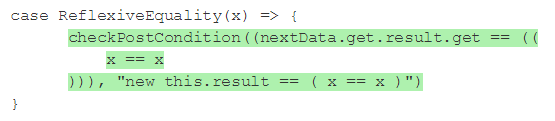
\includegraphics[width=\linewidth]{figures/eval_e0_reflexive-equality}
}
\caption{Test coverage example for \textit{ReflexiveEquality}}
\label{fig:ch3_eval_e0_highlighting_reflexive-equality}
\centering
\end{figure}
\FloatBarrier
% End figure
\pinfo{Property coverage}
The logic of a specification is defined in one Class in the generated system, which is called \textit{Logic} and prefixed by the specification name. We will only look at these classes to check to which extent the properties have been tested, using the highlighting that shows the coverage.\\
\\
\pinfo{Won't reach 100\%}
The generated system also contains some other logic that is more related to how it communicates with other instances when it is deployed, which is not something that we test. As a result, we will not be able to bring the test coverage to 100\%. However, all files in the generated system will be used to determine the overall coverage percentage. Since we use the same SUT to determine the coverage of the test suite on the SUT, the higher the coverage, the more complete it tests the defined properties in the generated system.

% Amount of bugs
\subsubsection{Amount of bugs}
\pinfo{Not a hard criteria, still using for indication}
The number of bugs found by an experiment also describes how effective the experiment was. Although this can not be a hard criteria, as it can vary per case. Consider that the system was already tested thoroughly, such that the bugs that this test suite would have found are already solved. This would mean that the amount of bugs found would remain 0, thus wouldn't have any effect as criteria. It is still an interesting part, as the amount of bugs found proofs that the test suite is able to find bugs. Because of this, we will report on this criteria and take it into account, but it will not be a critical criteria on determining whether one experiment was more successful than the other.

%\todo[inline]{Efficiency? Not yet.\\
%Can be done like getting coverage of libraries too, then substitute amount of properties and show that the same coverage can be received with less property tests. Thus less test cases, faster speed, same coverage. However, this would entail that the amount of bugs could go lower, as certain specific properties wont be tested if we require only coverage.}


% % % % % % % % % % % % % % % % % % % % % % % % % % % % % % % % % % % % %
% Section: Conclusion
\section{Conclusion}
\pinfo{Our approach, like QuickCheck}
The research question for this chapter lead as follows:\rqTwo{}. Existing approaches often require the SUT to be written in the same language. This was not possible when testing the generator in our case. The generator is being used to generate a system that is being used to test the generator. We use an approach that is similar to QuickCheck but using a \textit{Rebel} specification and the generated system to check whether the properties hold when using the generator.\\
\\
\pinfo{Combining all steps}
We demonstrated a full cycle based on one property, which indicated that this approach works to check a property. A full cycle consists of the following 5 phases:
\begin{enumerate}
\item \tfPhaseOne{}
\item \tfPhaseTwo{}
\item \tfPhaseThree{}
\item \tfPhaseFour{}
\item \tfPhaseFive{}
\end{enumerate}
The first step is done manually by translating the properties to a consistent \textit{Rebel} specification. The test framework is able to execute the other phases, which can be found in the \code{Main.rsc} file in the source code of this project.\\
\\
\pinfo{Larger specification for experiments}
For the experiments all the properties defined in \autoref{cpt:properties} will be used. This results in a bigger specification which can be used to test the generator automatically by using the test framework. After running the test framework, we evaluate it on the coverage and amount of bugs found metrics. The event definitions of each property defined in \autoref{cpt:properties} can be found in \autoref{app:a_event_definitions}.

% % % % % % % % % % % % % % % % % % % % % % % % % % % % % % % % % % % % %
% Section: Threats to validity
\section{Threats to validity}

\subsection*{Uncompilable system}
When the SUT is unable to compile, the test framework cannot proceed. As it cannot run the generated test suite against the SUT in that case. Although such errors could be detected by the test framework, it is out of scope for this thesis. IT is hard to argue whether the compilation error would be a bug or something else, as it can have many causes. However, when running the test framework this might still occur, which is a threat to this approach.

\subsection*{Accuracy}
\pinfo{Possibly incorrect results, due to Scoverage}
To evaluate the test framework we use coverage as a metric, which could have reported incorrect results. Scoverage is being used to determine the coverage and to generate a report from it. Since we are using random data as input, the results of the test coverage can fluctuate by small amounts in each run. However, we can still reason about the differences when there is a big difference between certain experiments. Additionally to the coverage we used the number of bugs that were found as another metric. This metric depends on which system the test suite is being run and if the system already fixed the bugs that the test suite would find. It is also the case that after fixing the bugs that were found earlier, this metric can be seen as unnecessary, as it would result in 0 then.

\subsection*{One system}
\pinfo{Only one generator}
Only one generator is being used throughout this thesis. However, it could be useful to make the test framework compatible with the other generators and generated systems too. This enables reasoning about the different implementations and its generators. Some changes are required to make the test framework compatible with these systems. But by doing so, every generated system for which a generator is built by ING can be checked based on the same properties, resulting in that the defined properties are checked thoroughly on every system and that inequalities can be detected between the different generators.\\
\\
\pinfo{Probably causing compile errors}
A threat in doing so is that one of the other generators might not support some translations of each expression that is used in the specification that we created. Thus this test framework can also be used to check whether every expression variant is taken into account by the generator. Unfortunately, an error in this translation would be blocking, in that it can lead to a generated system that is not able to compile. Resulting in that the test framework cannot proceed to run the test suite on the generated system. This could be used as a way to check the generators too. Although compilation errors were not the aim of the project, as compilation errors can have many causes, the test framework can still be used to detect those to a certain extent.

\subsection*{Whitebox implementation}
\pinfo{ScalaCheck, not testing generator then}
We chose to use property-based testing and implement the required functionality ourselfes, resulting in a white-box implementation. This means that we expect that our values generation is working correctly too. In case this isn't working correctly, this has to be fixed too.\\
\\
Another way how this could be done was to check how the custom types were generated to \textit{Scala}. And then generate a \textit{Scala} test project using the same types. Writing property tests for each type could achieve the same goal when it comes to checking the implementation of this component in the generated system. However, if we would follow this approach, we wouldn't use the generator to translate the \textit{Rebel} expressions to \textit{Scala}. This results in that the generator itself is still not being tested. With our approach, we test the generator and are able to find errors in the generator. Although we cannot conclude that the generator is implemented correctly if the generated test suit runs successful, rather we can conclude that the properties it checks for are satisfied.
